\chapter{Апробация}

В данном разделе будут проанализированы преимущества и недостатки разработанного решения. Также будет описана стратегия проверки корректности работы разработанного механизма классов типов, включающая в себя этапы, как автоматического, так и ручного тестирования. Стоит также отметить, что в рамках данной работы не рассматривалось нагрузочное тестирование разработанного механизма, а также не проверялась его совместимость с языком программирования Java. 

\section{Анализ разработанного решения}

Реализованный механизм, кажется, предоставляет пользователю всю необходимую для работы с классами типов функциональность: объявление классов типов и их экземпляров, ограничение принадлежности типовой переменной классу типов, а также вызов функций классов типов в контексте неизвестных на этапе исполнения значений типовых переменных. Полученное решение, конечно, нельзя назвать оптимальным даже в отношении синтаксиса использования классов типов, тем не менее оно дает достаточно полное представление о том, как концепция классов типов может быть интегрирована в язык программирования Kotlin. 

Ключевым элементом разработанного решения является модифицированный алгоритм разрешения вызовов функций, который может использовать значения типовых переменных для вычисления некоторых аргументов. Легко видеть, что почти вся функциональность, предоставляемая механизмом классов типов, обеспечивается именно этим алгоритмом. 

Среди недостатков разработанного подхода можно перечислить следующие:
\begin{enumerate}
    \item \label{it:flaw-6} В рамках разработанного решения допускается объявление экземпляров классов типов только в виде объектов. Это не позволяет описать экземпляр класса типов для параметризованных типов, в которых не указаны точные значения типовых переменных. Другими словами, например, не представляется возможным объявить экземпляр класса типов для обобщенного списка. Также данное ограничение требует от пользователя особого внимания в случае, когда экземпляры классов типов используются в нескольких потоках, а также при введении изменяемого состояния.  
    \item \label{it:flaw-5} Несмотря на то, что в область определении аннотации \code{@TypeClass} входят типовые переменные, ее использование в списке типовых переменных, который не относятся к функциям, игнорируется. 
    \item \label{it:flaw-4} Не допускается наследование между классами типов. % Данное решение было принято еще на этапе разработки требований и объяснялось тем, что в противном случае нельзя гарантировать уникальность экземпляров классов типов. Несмотря на то, что формально такое решение все еще считается необходимым, оно не допускает некоторые сценарии использования классов типов, которые могли бы быть корректно разрешены с соблюдением требования уникальности.  
    \item \label{it:flaw-1} Областью поиска экземпляров классов типов является вся программа. На первый взгляд, это не является критической проблемой, однако при ближайшем рассмотрении можно заметить, что зависимость вызова функции от некоторого экземпляра класса типов не выражена нигде в явном виде. Другими словами, пользователь в общем случае не может знать достоверное местоположение объявление интересующего его экземпляра класса типов.  
    \item \label{it:flaw-2} Способ включения экземпляров классов типов, определения которых встречаются в сторонних библиотеках, в список доступных экземпляров внутри программы также может затруднять понимание кода, поскольку разработанный механизм никаким образом не ограничивает места программы, в которых эти включения могут быть описаны. 
    \item \label{it:flaw-3} Неявные аргументы, играющие роль словарей функций классов типов, которые генерируются компилятором для функций, использующих классы типов, доступны для использования в теле таких функций в явном виде. С одной стороны, в этом нет никакой проблемы, однако исходный код, использующий эти неявные переменные напрямую может быть сложен для понимания. К тому же, разработанный механизм предоставляет пользователю доступ к этим переменным через вызов функции \code{dictionaryOf}. 
\end{enumerate}
Недостатки под номерами~\ref{it:flaw-1}, \ref{it:flaw-2} и \ref{it:flaw-3} могут быть устранены путем введения правил кодирования, которые строго регламентируют места описания и включения экземпляров классов типов, а также при достаточном уровне поддержки со стороны интегрированной среды разработки. Заметим, что недостатки~\ref{it:flaw-4} и \ref{it:flaw-5} также не представляются существенными, поскольку в контексте классов типов они ограничивают только лишь форму представления комбинаций классов типов. Стоит отметить, однако, что запрет наследования между классами типов может сказаться при использовании их в явном виде, как обычных типов.  Наиболее критическим здесь представляет первое ограничения, поскольку оно существенно сужает область применимости представленного алгоритма.    

\section{Тестирование}

Почти все модификации компилятора, представленные в предыдущем разделе, затрагивают только ту его часть, которая отвечает за анализ исходного кода программы. Исключение здесь составляет генерация байт-кода функций-делегатов, обеспечивающих доступ к функциям классов типов. При этом большинство разработанных алгоритмов необходимы для поддержания процесса разрешение вызовов функций, использующих классы типов. Напомним, что разрешение вызовов в компиляторе происходит уже после анализа всех деклараций, встречающихся в исходном коде программы, и, следовательно, алгоритм разрешения вызовов, использующих классы типов, полагается на результаты работы всех других частей разработанного механизма. Таким образом, тестирование только лишь этого алгоритма уже представляется достаточным для того, чтобы с высокой степенью уверенности говорить о корректности работы всего механизма классов типов. Для тестирования процесса разрешения вызовов, использующих классы типов, было решено организовать автоматическое тестирование. Все другие аспекты работы разработанного механизма тестировались ручным образом. 

Также стоит отметить, что исходный код компилятора Kotlin поставляется вместе с набором тестов, который насчитывает более двадцати тысяч тестовых сценариев работы компилятора. Успешное выполнение этих тестов, в свою очередь, позволяет утверждать, что интегрированный механизм классов типов не влияет негативным образом на базовую функциональность компилятора. 

\subsection{Автоматическое тестирование}

Для реализации модульных тестов, проверяющих работу механизма разрешения вызовов, в компиляторе существует специальный класс \code{AbstractResolvedCallsTest}. Для всякого тестового метода, объявленного в наследниках этого класса, необходимо создать два файла. Первый содержит компилируемый исходный код и допускает использование специального выражения \code{<caret>} перед вызовами функций, а содержимое второго состоит из двух частей: копии содержимого первого файла и информации о разрешенных вызовах, помеченных выражением \code{<caret>}. Пример описания результата разрешения вызова в файлах второго типа представлен в листинге~\ref{lst:test-file-example}. Процесс исполнения тестов данного вида организован следующим образом:
\begin{itemize}
    \item Загружается и анализируется файл первого типа. Под анализом здесь подразумевается в точности первый этап работы компилятора.
    \item Для всякого вызова, помеченного выражением \code{<caret>}, из контекста связываний, который был получен в результате анализа, извлекаются экземпляры \code{ResolvedCall}. 
    \item Формируется строка, формат которой соответствует формату файла второго типа: вначале располагает содержимое файла первого типа, а затем --- информация о результатах разрешения вызовов, которая извлекается из полученных на предыдущем этапе экземпляров класса \code{ResolvedCall}. 
    \item Полученная таким образом строка сравнивает с содержимым файла второго типа.
\end{itemize}

\lstinputlisting[
    label={lst:test-file-example},
    caption={Пример описания результата разрешения вызова в разработанных тестовых случаях},
    style={kotlin}
]
{resources/06/16_test_file_example}  

Все разработанные в рамках данной работы тесты можно разбить на три группы по проверяемому ими аспекту разрешения вызовов, использующих классы типов:
\begin{enumerate}
    \item Вычисление экземпляра класса типов для конкретных типов.
    \item Поиск подходящего словаря функций в случае, когда экземпляр класса типов не может быть вычислен.  
    \item Генерация объявлений функций-делегатов, обеспечивающих доступ к функциям класса типов.  
\end{enumerate}
Стоит отметить, что тестирование первого и второго аспектов также позволяет покрыть основные сценарии использования функции \code{dictionaryOf}.

Для тестирования первого аспекта использовалась иерархия типов, представленная на рисунке~\ref{fig:testing-hierarchy}, в которую укладываются все члены классов типов, определенных в рамках разработанных тестовых сценариев. Здесь стоит отметить, что, помимо типов, изображенных на рисунке~\ref{fig:testing-hierarchy}, в рамках данной иерархии допускается использование обнуляемых типов (nullable types). Заметим также, что в данной иерархии присутствует класс с множественным наследованием, что позволяет проверить корректность работы алгоритма вычисления экземпляров классов типов в случае существования более одного оптимального решения. Для удобства в дальнейшем будем ссылать на эту иерархию по номеру рисунка, на котором она изображена. Для формирования набора тестовых сценариев использовались следующие параметры:
\begin{itemize}
    \item Число типовых переменных в определении класса типов. Рассматривались случаи одной и трех типовых переменных. 
    \item Вариантность типовых переменных. Были рассмотрены случаи, в которых все типовые переменные имеют один из трех возможных модификаторов вариантности, а также одна случайная комбинация всех трех модификаторов в случае использования нескольких типовых переменных. При этом не проводилось различия между тем, объявлен ли модификатор вариантности в определении класса типов или в ограничении на типовую переменную.    
    \item Бинарный параметр, который определяет, указываются ли значения типовых переменных в точке вызова параметрически полиморфной функции или они должны быть вычислены из значений аргументов и/или типа возвращаемого значения.  
\end{itemize}

\begin{figure}[htbp]
    \centering
    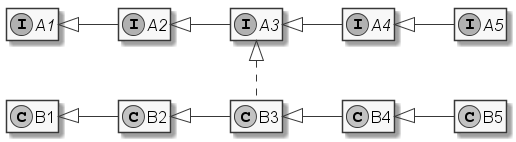
\includegraphics[width=\textwidth]{resources/07/02_testing_hierarchy.png}
    \caption{Иерархия типов, допустимых для использования в качестве членов классов типов в рамках тестовых сценариев}
    \label{fig:testing-hierarchy}
\end{figure}

Для всякой комбинации этих параметров был разработан тестовый случай, для каждого из которых, в свою очередь, объявляются класс типов и несколько его экземпляров для типов, входящих в иерархию~\ref{fig:testing-hierarchy}. Затем определяется параметрически полиморфная функция, которая предполагает использование объявленного класса типов, и анализируются ее вызовы для некоторого набора значений типовых переменных из той же иерархии. Члены класса типов при этом выбираются таким образом, чтобы в иерархии~\ref{fig:testing-hierarchy} нашлись типы, для которых нет подходящего экземпляра класса типов. Среди анализируемых вызовов также рассматриваются такие, для которых экземпляр класса типов не может быть вычислен. Это позволяет проверить корректность не только непосредственно алгоритма вычисления экземпляров классов типов, но также и работы алгоритма разрешения вызовов в целом. Пример исходного кода для разработанного таким образом тестового случая представлен в листинге~\ref{lst:test-resolve}. Здесь рассматривается случай единственной контравариантной типовой переменной (маркер контравариантности указан в объявлении функции \code{test}) и одновременно анализируются как вызовы с явным указанием значений типовых переменных, так и вызовы, в которых значения типовых переменных должны быть вычислены. Стоит также отметить, что для краткости в данном примере было опущено объявление типов, формирующих иерархию \ref{fig:testing-hierarchy}. 

\lstinputlisting[
    label={lst:test-resolve},
    caption={Пример исходного кода для тестирования процесса разрешения вызовов, использующих классы типов},
    style={kotlin}
]
{resources/07/03_test_resolve_example}  

Теперь рассмотрим более подробно ситуацию, в которой экземпляр класса типов не может быть вычислен. Здесь представляются возможными два варианта:
\begin{enumerate}
    \item В программе отсутствует объявление подходящего экземпляра классов типов.  
    \item Вместо конкретного типа указана типовая переменная.  
\end{enumerate}
На данном этапе можно считать, что алгоритм разрешения вызовов исправно функционирует в первом случае, однако до сих пор не проверялась корректность его работы во втором. Напомним, что при использовании типовых переменных в качестве членов класса типов в некоторой точке вызова разработанный алгоритм предпринимает попытку поиска подходящего экземпляра класса типов в списке аргументов функции, внутри которой расположен рассматриваемый вызов. Для того, чтобы показать корректность работы этой части алгоритма разрешения вызовов, рассмотрим две параметрически полиморфные функции \code{f} и \code{g}, которые используют один и тот же класс типов и вызов функции \code{g} располагается в теле функции \code{f}. В рамках тестирования процесса поиска подходящего экземпляра класса типов были рассмотрены следующие варианты размещения вызова функции \code{g}:
\begin{itemize}
    \item Вызов функции \code{g} является единственным выражением в теле функции \code{f}, вокруг которого опущены фигурные скобки. 
    \item Тело функции \code{f} заключено в фигурные скобки. 
    \item Вызов функции \code{g} располагается внутри анонимной функции.
    \item Вызов функции \code{g} располагается в теле локальной по отношению к \code{f} функции. 
\end{itemize}
В каждом тестовом случае, покрывающем описанные выше варианты использования классов типов, определяется единственный класс типов \code{C} с одной типовой переменной. При этом в функции \code{g} всегда используется экземпляр класса типов \code{C} только для какой-нибудь одной вариантности его типовой переменой, в то время как функция \code{f} может быть одного из двух видов:
\begin{itemize}
    \item В функции \code{f} используются экземпляры класса типов \code{C} для всех вариантностей его типовой переменной.
    \item В функции \code{f} используется только инвариантный по отношению к своей типовой переменной экземпляр класса типов \code{C}.
\end{itemize}
Для каждого вида функции \code{f} и каждой вариантности типовой переменной класса типов \code{C}, используемой в \code{g} был разработан тестовый случай. Таким образом, наличие двух видов функции \code{f} позволяет протестировать не только непосредственно поиск подходящего экземпляра класса типов, но также и работу алгоритма в случае, когда подходящий экземпляр не может быть вычислен или найден. Пример исходного кода, разработанного для тестирования одного из тестовых сценариев представлен в листинге~\ref{lst:test-search}. В данном примере в качестве \code{f} используется функция \code{testAnonymous}, а в роли \code{g} выступает функция \code{covariant}. Таким образом, здесь рассматривается случай, ковариантной типовой переменной и вызова \code{g}, расположенного внутри анонимной функции.  

\lstinputlisting[
    label={lst:test-search},
    caption={Пример исходного кода для тестирования алгоритма поиска экземпляра класса типов в случае, когда он не может быть вычислен},
    style={kotlin}
]
{resources/07/04_test_search_example}  

Рассмотрим теперь процесс тестирования механизма генерации объявлений функций-делегатов, обеспечивающих доступ к функциям класса типов. Сразу же отметим, что, поскольку исполнение тестов, проверяющих работу процесса разрешения вызовов, затрагивает только этап анализа исходного кода программы, здесь не представляется возможным проверить корректность генерации байт-кода соответствующих функций. Таким образом, следует сосредоточиться именно на механизме генерации определений функций-делегатов классов типов. Заметим, что функции-делегаты в классах типов являются параметрически полиморфными функциями и, следовательно, для тестирования корректности их генерации можно использовать тестовые сценарии, которые были описаны на этапе анализа алгоритма вычисления экземпляров классов типов с поправкой на то, что в рассматриваемом случае не допускается управление вариантностью типовых переменных класса типов нигде, кроме как в его определении. Для простоты было также решено ограничиться случаем рассмотрения нескольких типовых переменных, однако ввести дополнительный бинарный параметр, который указывает на то, присутствует ли в исходном коде уже объявленный объект-компаньон класса типов. Такой подход, однако, покрывает только те случаи, в которых функция-делегат может быть сгенерирована, что невозможно в случае, когда в объекте-компаньоне класса типов присутствует пользовательская функция с сигнатурой, идентичной сигнатуре функции-делегата. Такой вариант использования классов типов также был включен в список тестовых сценариев. 

\subsection{Ручное тестирование}

Целью ручного тестирования в рамках данной работы является проверка корректности функционирования частей разработанного механизма классов типов, которые не рассматривались на этапе автоматического тестирования, а также дополнительная проверка работоспособности компилятора после внесенных изменений. Для этих целей было разработано несколько простых программ, насчитывающих не более нескольких десятков классов. 

При проведении ручного тестирования особое внимание уделялось следующим аспектам разработанного механизма:
\begin{itemize}
    \item Генерация байт-кода функций-делегатов, обеспечивающих доступ к функциям классов типов.
    \item Использование классов типов и их экземпляров, определенных в сторонних библиотеках.
\end{itemize}
Проверка корректности работы обоих этих аспектов не представляет большой сложности. Генерация байт-кода функций-делегатов классов типов никаким образом не зависит ни от сигнатуры самой функции, ни от определения класса типов: здесь необходимо лишь гарантировать определенный порядок аргументов, однако это проверяется автоматическими тестами. Таким образом, корректность генерации байт-кода функций-делегатов классов типов может быть проверена на примере единственной функции. Для тестирования второго аспекта необходимо проверить, что при импортировании экземпляра класса типов, определенного в сторонней библиотеке, он будет учитываться при разрешении вызовов функций, в которых используется соответствующий класс типов. Программы, позволяющие проверить данный механизм в ручном режиме могут быть построены аналогично тестовым сценариям, использованным на этапе тестирования алгоритма вычисления подходящего экземпляра класса типов. Также стоит удостовериться в том, что отсутствие импорта также влияет на результат.